\documentclass{beamer}
\usetheme{Frankfurt}
\usecolortheme{dove}
\usepackage{arabtex}
%\usefonttheme{structuresmallcapsserif}
\setbeamercolor{section in head/foot}{fg=white, bg=black}

\makeatletter
\setbeamertemplate{footline}
{
  \leavevmode%
  \hbox{%
  \begin{beamercolorbox}[wd=.3 \paperwidth,ht=2.25ex,dp=1ex,center]{section in head/foot}%
    \usebeamerfont{author in head/foot}\insertshortauthor~~\beamer@ifempty{\insertshortinstitute}{}{(\insertshortinstitute)}
  \end{beamercolorbox}%
  \begin{beamercolorbox}[wd=.4\paperwidth,ht=2.25ex,dp=1ex,center]{section in head/foot}%
    \usebeamerfont{title in head/foot}\insertshorttitle
  \end{beamercolorbox}%
  \begin{beamercolorbox}[wd=.3\paperwidth,ht=2.25ex,dp=1ex,right]{section in head/foot}%
    \usebeamerfont{date in head/foot}\insertshortdate{}\hspace*{2em}
    \insertframenumber{} / \inserttotalframenumber\hspace*{2ex} 
  \end{beamercolorbox}}%
  \vskip0pt%
}
\makeatother

\begin{document}


\title{An Introduction to Econometric Software}
\subtitle{Session Three: \LaTeX{} and Git Hub}
\author{Charles Rahal}
\institute{charlierahal at gmail.com}
\date{\today}

\frame{\titlepage} 

\section{One}\label{one}
\subsection{Introduction and Pro\TeX t}
\frame{\frametitle{Course Admin - This Session: \LaTeX}
\begin{itemize}
\item This session will be slightly different from the others\\[0.1in]
\item What we will do is have two files open concurrently.\\[0.1in]
\item The first one will be these slides, which will contain all of the necessary commands.\\[0.1in]
\item The second one will be a text file (which we will save as a \emph{.tex} and `compile').\\[0.1in]
\item Hopefully then, by the end of the session, you will have created something similar to the file on Canvas '\emph{ourfirsttexfile.pdf}'.\\[0.1in]
\end{itemize}
}



\frame{\frametitle{Course Admin - This Session: GitHub}
\begin{itemize}
\item GitHub is a distributed revision control and source code management (SCM) system with an emphasis on speed, data integrity, and support for distributed, non-linear workflows.\\[0.1in]
\item Designed and originated by Linus Torvalds, the founder of the Linux Kernel, in April 2005 (as a successor/competitor to BitKeeper)\\[0.1in]
\item We will (briefly - although you must learn more about this independently) see how we can use it to host our code files.\\[0.1in]

\end{itemize}
}


\frame{\frametitle{Outline: \LaTeX}
\begin{itemize}
\item Section \ref{one}: Introduction and Pro\TeX t\\[0.1in]
\item Section \ref{two}: Article Class \\[0.1in]
\item Section \ref{three}: Structuring\\[0.1in]
\item Section \ref{four}: Text \\[0.1in]
\item Section \ref{five}: Mathematical Formulae\\[0.1in]
\item Section \ref{six}: Figures \\[0.1in]
\item Section \ref{seven}: Tables \\[0.1in]
\item Section \ref{eight}: Brief Intro to Bib\TeX{}\\[0.1in]
\end{itemize}
}

\frame{\frametitle{Introduction to \LaTeX}
\begin{itemize}
\item \LaTeX{}  ($\backslash$LaTeX) is a document preparation system and document markup language.\\[0.1in]
\item Based on \TeX{} ($\backslash$TeX), a typesetting system designed by Donald Knuth, released in 1978.\\[0.1in]
\item \LaTeX is not the name of any one particular program:\\
{\setlength\itemindent{25pt} 
\item It refers to encoding or tagging conventions used.}\\[0.1in]
\item Originally started out primarily the tool of mathematicians and scientists...
{\setlength\itemindent{25pt} 
\item But wider use has lead to the development of a very mature `programming' language
\item Prevalent in all of academia, but more-so in technical subjects.}
\end{itemize}
}

\frame{\frametitle{Introduction to \LaTeX (Cont.)}
\begin{itemize}
\item Popular for its ability to elegantly handle equations:
\begin{equation}
y_{t+H}=\alpha_y+\Phi_y (L) y_t + \Phi_x (L) x_t^i + \varepsilon_{y,t+H}
\end{equation}\\[0.1in]
\item One of the main features of \LaTeX{} is the ability to write a range of complex characters.\\[0.1in]
\item For example, maybe we want to write Arabic?\\
\begin{center}
\setcode{utf8}
\RL{السَلامُ عَليكم ورَحمةُ الله وبَركاته}
\end{center}
\end{itemize}
}

\frame{\frametitle{Introduction to \LaTeX (Cont.)}
But what does \LaTeX{} actually look like?
\begin{figure}
    \scalebox{.2}{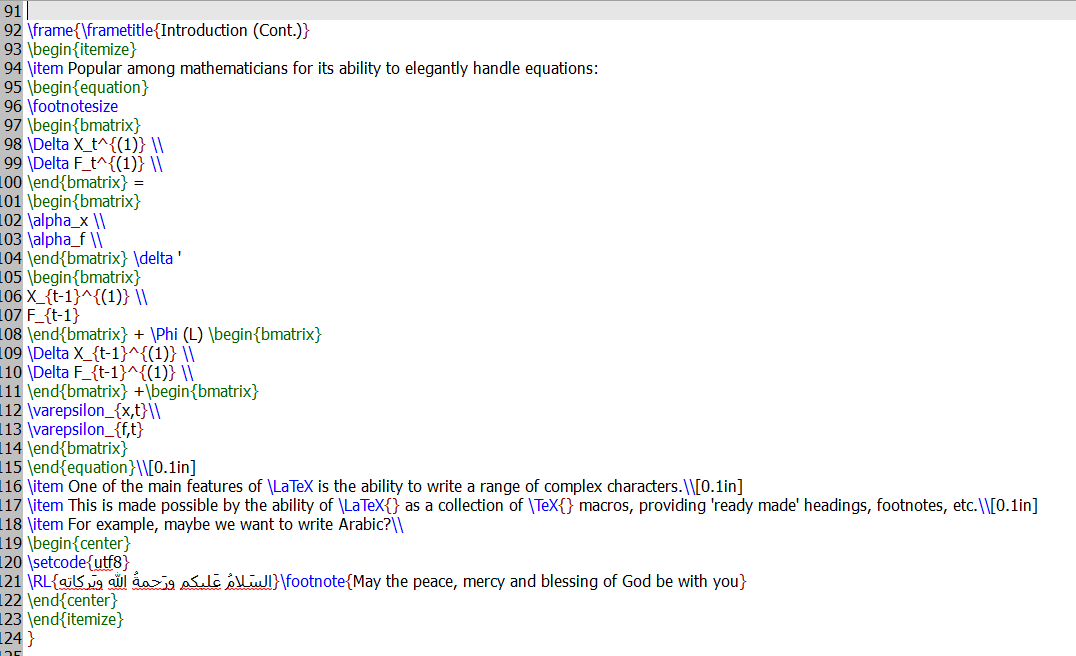
\includegraphics{texexample.png}}
\end{figure}
\begin{itemize}
\item The aim of today will be to get you towards being able to produce something like this (but in the \emph{article} class variety).\\
\item However! We will not be discussing the technicalities of the compilation process or production of \emph{.gz}, \emph{LOG} or \emph{.aux} files.\\
\end{itemize}
}

\frame{\frametitle{Introduction (Cont.)}
Disadvantages of \LaTeX{}, compared to a \color{red} \href{http://en.wikipedia.org/wiki/WYSIWYG}{WYSIWYG}\footnote{Note! You can click this word! Created using the package \small \textbf{hyperref} \normalsize package \\[0.025in]} \color{black} program such as MS Word:\\[0.1in]
\begin{enumerate}
\item You are unable to see the results instantly.\\[0.1in]
\item There is a learning curve as in any code language regarding the vocabulary of basic commands.\\[0.1in]
\item It can often be difficult to generate a specific `look' or `feel'.\\[0.2in]
\item The debugging process can be frustrating, to say the least!\\
\end{enumerate}
}

\frame{\frametitle{Introduction (Cont.)}
However, as a \color{red} \href{http://en.wikipedia.org/wiki/WYSIWYM}{WYSIWYM} \color{black} language, the benefits are enormous:\\
\begin{enumerate}
\item Layouts, fonts, tables are consistent throughout.\\[0.1in]
\item Formula are especially easy to typeset beautifully.\\[0.1in]
\item Indices, footnotes and other references are easily generated.\\[0.1in]
\item Your documents will have a correct systematic structure.\footnote{For example, open these slides in Adobe Reader IX or many other \emph{.pdf} viewers to see the section headings in the left hand side\\}\\[0.1in]
\item It is \color{purple}\textbf{FREE!} \color{black}\\[0.1in]
\item It is cross-platform: Any \emph{.tex} file can be compiled through any compiler on any operating system.\\
\end{enumerate}
}

\frame{\frametitle{ProTeXt}
\begin{itemize}
\item The most popular windows distribution of \TeX{}:\\[0.1in]
\end{itemize}
\begin{center}
\url{www.tug.org/protext/}\footnote{This is created using the $\backslash$url\{\}	 command\\}
\end{center}
\begin{itemize}
\item Alternatively: TeX Live for Unix/GNU/Linux:
\begin{center}
\texttt{sudo apt-get install texlive}\\[0.1in]
\end{center}
\item If you want some help installing ProTeXt, stick around after the class either here or in MHT 7W.\\[0.1in]
\item Today we'll be working out of GUI TeXworks - a free open source program with an integrated viewer packaged in the proTeXt distribution.\\[0.1in]
\end{itemize}
}

\frame{\frametitle{Best Free Manual}
\begin{itemize}
\item A free e-book has emerged over time as the leading standard:\\
\begin{figure}
    \scalebox{.45}{
\includegraphics{freelatexbook.png}}\\[0.2in]
\end{figure}
\item This is the book that we will largely follow (\emph{very}) loosely.\\
\item You can find it at: \url{https://tobi.oetiker.ch/lshort/lshort.pdf}.
\end{itemize}
}

\section{Two}\label{two}
\subsection{Article Class}
\frame{\frametitle{Our First \LaTeX{} document}
Lets create our first \LaTeX{} document\footnote{Note: all \LaTeX{} commands \tt{{are written like this - $\backslash$texttt\{\}}}.\\}.\\[0.2in]
\begin{tt}
$\backslash$documentclass[a4paper, 12pt]\{article\}\\
\% This is just one of many available `classes'\\
$\backslash$begin\{document\}\\
\% Begin/end document prefix and suffix all documents.\\
Hello World!\\
$\backslash$end\{document\}\\[0.2in]
\end{tt}
Note that options for the document class are specified in [$\cdot$].
}

\frame{\frametitle{Some Introductory Points to Note}
\begin{itemize}
\item Note that we are `commenting out' with the \% command, e.g.:\\[0.2in]
\begin{center}
\begin{tt}
This is an \% extremely\\
\% unnecessarily complicated\\\
example: Supercal\%\\
ifragilist\%\\
icexpialidocious\\
\end{tt}
\end{center}
\end{itemize}
\begin{block}{Commenting Out}
This is an % stupid
% Better: instructive <----
example: Supercal%
ifragilist%
icexpialidocious
\end{block}
}









\frame{\frametitle{Some Introductory Points to Note}
\begin{itemize}
\item We might note at this point the difference between ' and ` \\
\item And the use of the `$\backslash$hdots' command...\\[0.2in]
\end{itemize}
Some special commands such as inserting \% are as follows:\\
\begin{figure}
    \scalebox{.75}{\includegraphics{specialcharacterslatex.png}}
\end{figure}
}

\frame{\frametitle{Front Matter}
\begin{itemize}
\item After \begin{tt}$\backslash$begin\{document\}\end{tt}, we have \begin{tt}frontmatter \end{tt}.\\[0.2in]
\item \texttt{frontmatter} contains things such as:
\begin{enumerate}
\item  \begin{tt}$\backslash$title\{$<$\emph{TITLE}$>$\}\end{tt}: Where \begin{tt}<\emph{TITLE}>\end{tt} is the title.\\[0.1in]
\item  \begin{tt}$\backslash$date\{$<$\emph{DATE}$>$\}\end{tt}: Inputs a specific date.\\[0.1in]
\item  \begin{tt}$\backslash$author\{$<$\emph{FIRST AUTHOR NAME\}$>$}\end{tt}: Insert your name here!\\[0.1in]
\end{enumerate}
\item We then need to tell \LaTeX{} to make the title with the command \begin{tt}$\backslash$maketitle\end{tt}.
\end{itemize}
}

%\item \tt{$\backslash$affiliation}\{<\emph{AFFILIATION}>\}: Your place of business!\\

\frame{\frametitle{Front Matter (Cont)}
Lets try it out - insert the following commands after $\backslash$begin\{document\}:\\[0.2in]
\begin{block}{Front Matter}
\begin{tt}
$\backslash$begin\{document\}\\
$\backslash$title\{My First $\backslash$LaTeX Document!\}\\
$\backslash$date\{01/11/2013\}\\
$\backslash$author\{Charlie Rahal\}\\
$\backslash$maketitle\\
\end{tt}
\end{block}
}

\frame{\frametitle{Front Matter (Cont)}
\begin{itemize}
\item It might be rational for us to want to include our contact information.\\
\item One way which we could do this would be to split up the $\backslash$author section (note the use of $\backslash$$\backslash$ to create line-breaks):
\end{itemize}
\begin{block}{Front Matter}
\begin{tt}
$\backslash$author\{Charlie Rahal$\backslash$$\backslash$\\
Department of Economics,$\backslash$$\backslash$\\
UoB,$\backslash$$\backslash$\\
Birmingham.$\backslash$$\backslash$\\
\href{mailto:cxr828@bham.ac.uk}{cxr828 at bham.ac.uk}\}\\
$\backslash$maketitle\\
\end{tt}
\end{block}
}

\frame{\frametitle{Preamble}
\begin{itemize}
\item How did we make it so that you can click the e-mail address on the previous page?\\[0.1in]
\item Or so that the links \color{red}\href{http://en.wikipedia.org/wiki/WYSIWYM}{WYSIWYM} \color{black} and \color{red} \href{http://en.wikipedia.org/wiki/WYSIWYG}{WYSIWYG} \color{black} were clickable?\\[0.1in]
\item The solution lies in including the package (not a default inclusion) in \LaTeX{} in the \emph{preamble}.\\[0.1in]
\item The \emph{preamble} is the section \textbf{before} the \begin{tt}$\backslash$begin\{document\}\end{tt}.\\[0.1in]
\end{itemize}
For example, include:\\
\begin{center}
\begin{tt}
$\backslash$usepackage\{hyperref\}
\end{tt}
\end{center}
And change the e-mail address in the \emph{frontmatter} to:
\footnotesize
\begin{center}
\begin{tt}
$\backslash$href\{mailto:CXR828@bham.ac.uk\}\{cxr828 at bham dot ac dot uk\}
\end{tt}
\end{center}
}

\frame{\frametitle{Abstract}
\begin{itemize} 
\item It is entirely likely that if we are using the article class, we are going to need an abstract.\\[0.1in]
\item To do this, we simply use the command \begin{tt}$\backslash$begin\{abstract\} and $\backslash$end\{abstract\}\end{tt}.\\[0.1in]
\item Let's put it just below the \begin{tt}$\backslash$maketitle\end{tt} command:\\[0.2in]
\end{itemize}
\begin{block}{An Abstract}
$\backslash$begin\{abstract\}\\
This is an abstract which details the creation of our first adventures with \LaTeX.\\
$\backslash$end\{abstract\}
\end{block}
}
\frame{\frametitle{Summary So Far}
Hopefully, you have been following along with the slides and have got something which looks like this:\\[0.1in]
\begin{figure}
    \scalebox{.65}{
\includegraphics{titlepage.png}}
\end{figure}
}

\frame{\frametitle{Breaks}
\begin{itemize}
\item We will often want to start fresh pages for different sections:\\
\begin{center}
\begin{tt}
$\backslash$newpage\\
\end{tt}
\end{center}
\item Let's start a new page after our abstract.\\[0.1in]
\item At this point, note that an empty line starts a new paragraph.\\[0.1in]
\item And \texttt{$\backslash\backslash$} or \texttt{$\backslash$newline} orders a line break.\\[0.1in]
\item \texttt{$\backslash\backslash^*$} starts a new line, prohibbiting a page break.
\end{itemize}
}

\section{Three}\label{three}
\subsection{Structuring}
\frame{\frametitle{Structure}
\begin{itemize}
\item One of the best features of \LaTeX{} is the way you can add structure to your documents.\\[0.1in]
\item Lets add the Sections Corresponding to the remainder of the class on our new page:\\[0.1in]
\end{itemize}
\begin{block}{Sections}
$\backslash$section\{Text and Characters\}\\
$\backslash$section\{The Beauty of Mathematics in \LaTeX\}\\
$\backslash$section\{Figures\}\\
$\backslash$section\{Tables\}\\
\end{block}
}




\frame{\frametitle{Structure (Cont.)}
\begin{itemize}
\item It is likely that we are also going to want to use subsections:
\end{itemize}
\begin{block}{Subsections}
$\backslash$section\{Text and Characters\}\\
$\backslash$subsection\{Bold\}\\
$\backslash$subsection\{Italics\}\\
$\backslash$subsection\{Typewritter\}\\
$\backslash$subsection\{Colors\}\\
$\backslash$subsection\{Underline\}\\
$\backslash$section\{The Beauty of Mathematics in \LaTeX\}\\
$\backslash$section\{Figures\}\\
$\backslash$section\{Tables\}\\
\end{block}
}


\frame{\frametitle{Structure (Cont.)}
\begin{itemize}
\item It is likely that we are also going to want to use subsubsections (See the .\TeX version of this .pdf to see how it's structured.)\\[0.1in]
\end{itemize}
\footnotesize
\begin{block}{Subsubsections}
$\backslash$section\{Text and Characters\}\\
$\backslash$subsection\{Bold\}\\
$\backslash$subsection\{Italics\}\\
$\backslash$subsubsection\{textit\}\\
$\backslash$subsubsection\{emph\}\\
$\backslash$subsection\{Typewritter\}\\
$\backslash$subsection\{Underline\}\\
$\backslash$subsection\{Colors\}\\
$\backslash$subsection\{Lists\}\\
$\backslash$section\{The Beauty of Mathematics in \LaTeX\}\\
$\backslash$section\{Figures\}\\
$\backslash$section\{Tables\}\\
\end{block}
}


\frame{\frametitle{Structure (Cont.)}
\begin{itemize}
\item Two final commands of interest in this section are:
\begin{center}
\begin{tt}
$\backslash$section*\{\}
\end{tt}
\end{center}
which is able to create un-numbered sections.\\[0.2in]
\item And we might also want to note for larger documents we would like to use \begin{tt}$\backslash$part \end{tt}or \begin{tt}$\backslash$chapter. \end{tt}\\[0.2in]
\item In particular, we will probably want to insert a table of contents after the abstract on the first page:
\begin{center}
\begin{tt}
$\backslash$tableofcontents
\end{tt}
\end{center}
\end{itemize}
}

\frame{\frametitle{Summary So Far}
Hopefully, you have been following along with the slides and have got something which looks like this:\\[0.1in]
\begin{figure}
    \scalebox{.2}{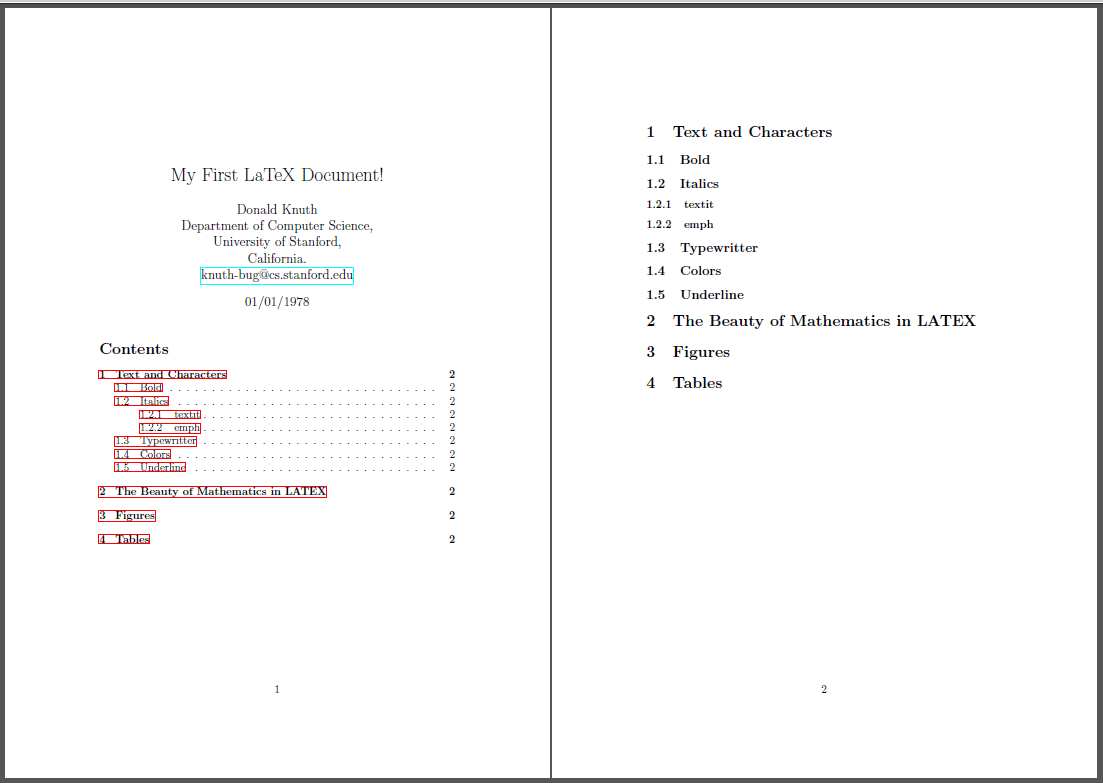
\includegraphics{withtoc.png}}
\end{figure}
}

\section{Four}\label{four}
\subsection{Text}
\frame{\frametitle{Bold}
\begin{itemize}
\item First of all, lets note that we can \textbf{include bold font}.
\item We normally do this with the command:\\
\begin{center}
\begin{tt}
$\backslash$textbf\{$<$insert bold text here$>$\}\\[0.1in]
\end{tt}
\end{center}
\item In our section on bold text, lets try:
\end{itemize}
\begin{block}{Bold}
\begin{tt}
Our first attempt at writing $\backslash$textbf\{SOMETHING IN BOLD!\}\\
\end{tt}
\end{block}
}

\frame{\frametitle{Italics (Cont.)}
\begin{itemize}
\item As you might expect from our subsubsections above, there are two ways to create \textit{italicized} text.\\
\begin{enumerate}
{\setlength\itemindent{1cm}
\item The first of which is the $\backslash$emph\{\} command:}\\
\begin{center}
\emph{This is written using $\backslash$emph\{\}}.\\
\end{center}
{\setlength\itemindent{1cm}
\item The second option we have is to use $\backslash$textit\{\}}:
\begin{center}
\textit{This is written using $\backslash$textit\{\}}.\\[0.2in]
\end{center}
\end{enumerate}
\item Add in these two lines to your \emph{myfirsttex.tex}.\\[0.2in]
\end{itemize}
}

\frame{\frametitle{Italics}
\begin{itemize}
\item \textbf{However}, be sure to note the difference - $\backslash$emph\{\} can be pre-defined in the pre-amble and can have different features (e.g. underline) in different classes.\\[0.2in]
\item Note the difference between $\backslash$textit\{\} and $\backslash$it\{\}:\\
{\setlength\itemindent{1cm}
\item $\backslash$it\{\} and $\backslash$bf\{\} and other similar commands are only supported for historical reasons: they do not nest well together:}\\[0.1in]
\begin{center}
$\backslash$it\{This is not in $\backslash$bf\{bold italics\}\}\\
\it{This is not in \bf{bold italics}}\\
\end{center}
\end{itemize}
}

\frame{\frametitle{Underline and Typewriter}
\begin{itemize}
\item Using similar logic to $\backslash$textit\{\} and $\backslash$textbf\{\}, we can also define $\backslash$underline\{\}. Let's put this in our document:
\begin{center}
\underline{This is underlined}\\[0.3in]
\end{center}
\item And we can also create 'typewriter font' which is what all of our \LaTeX{} commands in these slides are written in: $\backslash$texttt\{\}:
\begin{center}
\texttt{This is written in typewriter font.\footnote{Let's take this opportunity to create a footnote with the $\backslash$footnote\{\} command.\\}}\\[0.2in]
\end{center}
\end{itemize}  
}

\frame{\frametitle{Flushing}
\begin{itemize}
\item Note that on the previous slide, some of the text was left-aligned:\\
\begin{flushleft}
Created using \texttt{$\backslash$begin\{flushleft\}} and  \texttt{$\backslash$end\{flushleft\}}\\[0.2in]
\end{flushleft}
\item Some of it was centered:\\[0.1in]
\begin{center}
Using the \texttt{$\backslash$begin\{center\}} and \texttt{$\backslash$end\{center\}}.\\[0.2in]
\end{center}
\item And we could also right align if we wanted to:\\
\begin{flushright}
The \texttt{$\backslash$begin\{flushright\}} and  \texttt{$\backslash$end\{flushright\}}\\
\end{flushright}
\end{itemize}
}

\frame{\frametitle{Colours}
\begin{itemize}
\item To make use of colours, we must add a new package:\\
\begin{center}
\texttt{$\backslash$usepackage\{color\}}\\
\end{center}	
\item To write in colour we can use the command:\\
\texttt\{$\backslash$textcolor\{yourcolor\}\{yourtext\}\}.\\
or\\
\texttt\{$\backslash$textcolor\{yourcolor\}\{yourtext\}\}.\\
\item For example: \texttt\{$\backslash$color\{red\}\{this is written in red!\}\} gives us:\\
\begin{center}
\color{red}{this is written in red!}
\end{center}
\item We can change the page colour using the command:\\
\begin{center}
$\backslash$pagecolor\{yourpagecolor\}\\
\end{center}
\end{itemize}
}

\frame{\frametitle{Colours (Cont.)}
\begin{itemize}
\item We can also box colours - for example:
\begin{center}
\begin{tt}
$\backslash$colorbox\{red\}\{our red colorblock\}
\end{tt}
\end{center}
produces \colorbox{red}{our red colorblock}\\[0.2in]
\item In addition, we can add a color to the border:
\begin{center}
\begin{tt}
$\backslash$fcolorbox\{red\}\{green\}\{our green colorbox with red background\}
\end{tt}
\end{center}
produces \fcolorbox{red}{green}{our green colorbox with red background}
\end{itemize}
}

\frame{\frametitle{Lists}
\begin{itemize}
\item As you may have noticed, many of the slides in this course feature bullet points.\\[0.2in]
\item We can create bullet points with \texttt{$\backslash$begin\{itemize\}} and \texttt{$\backslash$end\{itemize\}}\\[0.2in]
\item Then we start new a \texttt{$\backslash$item} on each line.\\[0.2in]
\item To indent an item, use: \texttt\{$\backslash$setlength$\backslash$itemindent\{25pt\}\}.\\[0.1in]
{\setlength\itemindent{25pt} 
\item Where 25pt is the amount which we want to indent.}\\[0.1in]
\end{itemize}
} 

\frame{\frametitle{Lists (Cont.)}
\begin{itemize}
\item In particular, maybe we want to create a numbered list.\\[0.1in]
\item To do this, use the \texttt{$\backslash$begin\{enumerate\}}, but don't forget \texttt{end!}\\[0.1in]
\item Try an example in your working document:\\[0.2in]
\begin{block}{My favourite classes:}
\begin{enumerate}
\item Econometrics\\
\item Macroeconomics\\
\item Microeconomics\\
\end{enumerate}
\end{block}
\end{itemize}
}

\section{Five}\label{five}
\subsection{Mathematical Formulae}
\frame{\frametitle{Mathematical Formulae}
\begin{itemize}
\item One of the main strengths of \TeX{} is the ability to typeset formulae.\\[0.2in]
\item While \LaTeX{} will have some functionatlity installed, we are going to work with \AmS-\LaTeX :\\[0.2in]
{\setlength\itemindent{25pt} 
\item A collection of \LaTeX{} document classes and packages developed for the American Mathematical Society (AMS).}\\[0.2in]
\item We are going to want to load the package into the pre-amble:
\begin{center}
\begin{tt}
$\backslash$usepackage\{amsmath\}
\end{tt}
\end{center}
\end{itemize}
}

\frame{\frametitle{Mathematical Formulae (Cont.)}
\begin{itemize}
\item Mathematical formula can be set \emph{within} a paragraph (`text style'):\\
E.g.: $a^2+b^2=c^2$ is written with \$a\textasciicircum2+b\textasciicircum2=c\textasciicircum2\$.\\[0.2in]
\item If we wanted to set these equations apart like this (`display style'):
\begin{equation}
a^2+b^2=c^2
\end{equation}
then we need to use the $\backslash$begin\{equation\} and $\backslash$end\{equation\} commands.\\[0.1in]
\item Note the automatic generation of equation numbering, which can be suppressed with$\backslash$begin\{equation$^*$\}
\end{itemize}
}

\frame{\frametitle{Mathematical Formulae (Cont.)}
It is also possible to display more difficult equations such as:
\begin{equation}
\lim_{n \to \infty}
\sum_{k=1}^n \frac{1}{k^2}
= \frac{\pi^2}{6}
\end{equation}
Which we can create with:\\
\begin{block}{More advanced equations}
\texttt{
$\backslash$begin\{equation\}\\ 
$\backslash$lim\_\{n $\backslash$to $\backslash$infty\}\\
$\backslash$sum\_\{k=1\}\textasciicircum n $\backslash$frac\{1\}\{k\textasciicircum2\}\\
=$\backslash$frac\{$\backslash$pi\textasciicircum 2\}\{6\}\\
$\backslash$end\{equation\}
}
\end{block}
}


\frame{\frametitle{Mathematical Formulae (Cont.)}
We can add accents to any of our mathematical characters in math mode:
\begin{figure}
    \scalebox{.3}{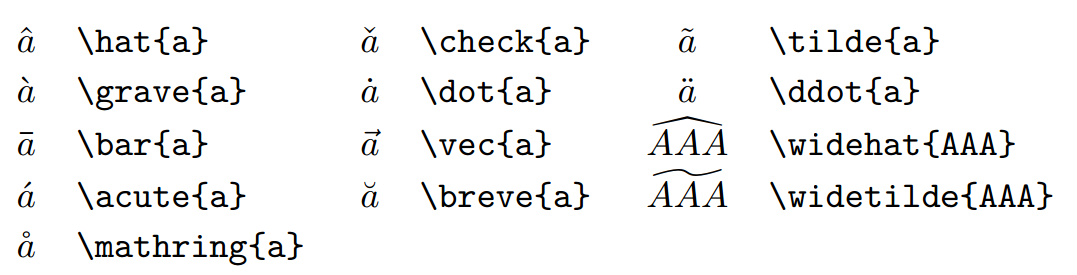
\includegraphics{accents.png}}
\end{figure}
Note that we can also include set letters such as: $\mathbb{N}$, $\mathbb{Z}$, $\mathbb{Q}$, $\mathbb{R}$, $\mathbb{C}$.
\begin{block}{Set Letters}
$\backslash$mathbb\{N\}, $\backslash$mathbb\{Z\}, $\backslash$mathbb\{Q\}, $\backslash$mathbb\{R\}, $\backslash$mathbb\{C\}
\end{block}
}


\frame{\frametitle{Mathematical Formulae (Cont.)}
Of particular importance is the use of \emph{arrays}
\begin{equation*}
\mathbf{X} = \left(
\begin{array}{ccc}
x_1 & x_2 & \ldots \\
x_3 & x_4 & \ldots \\
\vdots & \vdots & \ddots
\end{array} \right)
\end{equation*}
Which we can create with:\\[0.1in]
\begin{block}{Our First Array}
\small
\begin{center}
\texttt{
$\backslash$begin\{equation*\}\\
$\backslash$mathbf\{X\} = $\backslash$left(\\
$\backslash$begin\{array\}\{ccc\}\\
x\_1 \& x\_2 \& $\backslash$ldots \\
x\_3 \& x\_4 \& $\backslash$ldots \\
$\backslash$vdots \& $\backslash$vdots \& $\backslash$ddots\\
$\backslash$end\{array\}$\backslash$right)\\
$\backslash$end\{equation*\}\\	
}
\end{center}
\end{block}	
}

\frame{\frametitle{Mathematical Formulae (Cont.)}
And a similar variant of which is the matrix:
\begin{equation*}
\begin{matrix}
1 & 2 & 3 & 4 & 5 \\
6 & 7 & 8 & 9 & 10 \\
11 & 12 & 13 & 14 & 15\\
16 & 17 & 18 & 19 & 20\\ 
21 & 22 & 23 & 24 & 25 \\
\end{matrix} \qquad =
\begin{bmatrix}
p_{11} & p_{12} & \ldots
& p_{1n} \\
p_{21} & p_{22} & \ldots
& p_{2n} \\
\vdots & \vdots & \ddots
& \vdots \\
p_{m1} & p_{m2} & \ldots
& p_{mn}
\end{bmatrix}
\end{equation*}\\[0.2in]
Where the LHS is created with $\backslash$begin/end\{matrix\} and the RHS is created with $\backslash$begin/end\{bmatrix\}.\\
}

\frame{\frametitle{Mathematical Formulae (Cont.)}
The range of Greek letters which we can include is shown here:
\begin{figure}
    \scalebox{.3}{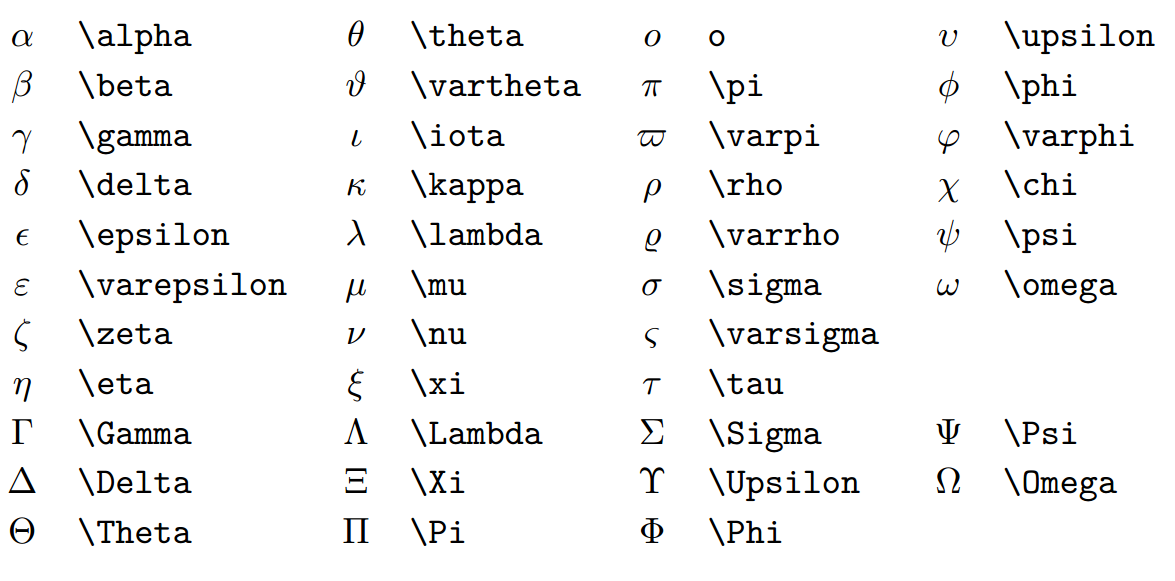
\includegraphics{greekletters.png}}
\end{figure}
Note the use of capital and lowercase letters
}


\section{Six}\label{six}
\subsection{Figures}
\frame{\frametitle{Inserting Figures}
\begin{itemize}
\item To insert a figure, we must use the $\backslash$begin\{figure\} command.\\[0.1in]
\item Note that we need to add a package: $\backslash$usepackage\{graphicx\}.\\[0.1in]
\item As an example, lets try it with the \color{red}cat \color{black}on \emph{Canvas}:\\[0.2in]
\begin{block}{Our First Figure}
\small
\begin{tt}
$\backslash$begin\{figure\}[!ht]\\
$\backslash$begin\{center\}\\
$\backslash$caption*\{Cat with Monocle\}\\
$\backslash$includegraphics[scale=0.3]\{cat\}\\
$\backslash$end\{center\}\\
$\backslash$end\{figure\}\\
\end{tt}
\end{block}
\end{itemize}
}

\frame{\frametitle{Inserting Figures (Cont.)}
\begin{figure}[!ht]
\begin{center}
\caption{\color{red}\textbf{Cat with monocle}}

\includegraphics[scale=0.2]{cat}
\end{center}
\end{figure}
}

\frame{\frametitle{Inserting Figures (Cont.)}
Lets review some of the commands in the previous slide.\\[0.1in]
\begin{itemize}
\item Caption can go above/ below the figure (includegraphics command), depending on whether you want it to go above/below.\\[0.1in]
\item The command [!ht] tells \LaTeX{} to try (!=try very hard) here [h] or at the top [t] if [h] is impossible.\\[0.1in]
\item The options in includegraphics[$\cdot$] generally relate to:  
{\setlength\itemindent{25pt} 
\item \emph{scale} such as we did.\\
\item \emph{width} or \emph{height} such as \begin{tt}width=$\backslash$textwidth \end{tt}\\
\item Or \emph{angle} which can change the rotation.}\\
\item Note that in our example, the aspect ratio is 1.0.\\
\end{itemize}
}

\section{Seven}\label{seven}
\subsection{Tables}
\frame{\frametitle{Tabular Environments}
The command underlying all of our tabular environs is:\\
\begin{tt}
\begin{center}
$\backslash$begin\{tabular\}[pos]\{table spec\}
\end{center}
\end{tt}
where [pos] is the position and \{table spec\} outlines all of the features of our table, specifically regarding the alignment to be used in each column and the vertical lines to insert.\\
\begin{table}
\caption{Options for column specification}
\begin{tabular}[!h]{c | c}
\hline
$l$ & left-justified column \\
$c$ & centered column \\
$r$ & right justified column \\
$p$\{'width'\} & paragraph column with text vertically aligned at top\\
\textbar  & vertical line down the columns\\
\hline
\end{tabular}
\end{table}
}

\frame{\frametitle{An example table}
The table on the last page is a bit more complicated than we need. Lets try something slightly simpler:\\
\begin{block}{Our First Table}
\begin{tt}
\footnotesize
$\backslash$begin\{center\}\\
\small
$\backslash$begin\{table\}\\
\small
$\backslash$caption\{Our First Table\}\\
\small
$\backslash$begin\{tabular\}[!h]\{c \textbar c \textbar c \textbar c \}\\
\small
Subject \& Difficulty \& Fun \& Usefulness$\backslash$$\backslash$$\backslash$hline\\
\small
Econometrics \& 10 \& 10 \& 10$\backslash$$\backslash$\\
\small
Finance \& 8 \& 9 \& 10$\backslash$$\backslash$\\
\small
Macroeconomics \& 9 \& 7 \& 9$\backslash$$\backslash$\\
\small
Microeconomics \& 7 \& 4 \& 1 $\backslash$ $\backslash$\\
\small
$\backslash$end\{tabular\}\\
\small
$\backslash$end\{table\}\\
\small
$\backslash$end\{center\}\\
\small
\end{tt}
\end{block}
} 

\frame{\frametitle{An example table(Cont)}
\begin{center}
\begin{table}
\caption{Our First Table}
\begin{tabular}[!h]{c | c | c | c }
Subject & Difficulty & Fun & Usefulness\\ \hline
Econometrics & 10 & 10 & 10\\
Finance & 8 & 9 & 10\\
Macroeconomics & 9 & 7 & 9\\
Microeconomics & 7 & 4 & 1\\
\end{tabular}
\end{table}
\end{center}
}

\section{Eight}\label{eight}
\subsection{Brief Intro to Bib\TeX{}}
\frame{\frametitle{An Introduction to Bib\TeX}
\begin{itemize}
\item Bib\TeX is a file format designed to work with La\TeX.\\
\item A Bib\TeX{} entry contains things like author name, journal title, etc:\\[0.1in]
\begin{footnotesize}
\begin{center}
\begin{tt}
@Article\{OlmoPouliot,\\
  author=\{Olmo Jose and Pouliot William\},\\
  title=\{Early Detection Techniques for Market Risk Failure\},\\
  journal=\{Studies in Nonlinear Dynamics \& Econometrics\},\\
  year=2011,\\
  volume=\{15\},\\
  number=\{4\},\\
  pages=\{1-55\},\\
  month=\{September\},\\
  keywords=\{\},\\
\}
\end{tt}
\end{center}
\end{footnotesize}
\end{itemize}
}

\frame{\frametitle{An Introduction to Bib\TeX (Cont.)}
\begin{itemize}
\item Let's note: \emph{@article} is the entry type (the type of publication).\\[0.1in]
\item \emph{OlmoPouliot} is called the \emph{identifier}.\\[0.1in]
\item \emph{author}, \emph{title}, etc all relate to what you might expect.\\[0.1in]
\item Some Bib\TeX{} entries also contain abstracts.\\[0.1in]
\item We can call it from BiB\TeX{} using $\backslash$cite\{\} command.\\[0.1in]
\item e.g. cite the paper by Dr. Pouliot using: $\backslash$cite\{OlmoPouliot\} $\hdots$\\
\end{itemize}
}

\frame{\frametitle{An Introduction to Bib\TeX (Cont.)}
\begin{itemize}
\item However, first we need to set up our \emph{.bib} file.\\[0.1in]
\item To do this, find a .bib reference from any of your favourite papers on IDEAS or google scholar or something similar.
\begin{figure}[!ht]
\begin{center}
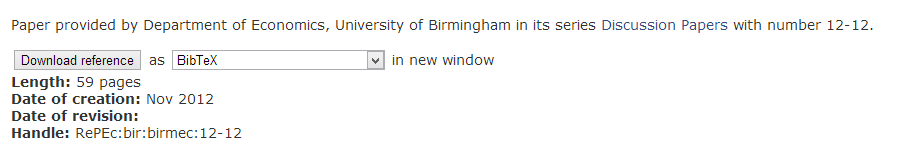
\includegraphics[scale=0.4]{bibtexexample}
\end{center}
\end{figure}
\item Then save this to a text file with the extension \emph{.bib} e.g.\emph{myfirstbib.bib}\\[0.1in]
\end{itemize}
}

\frame{\frametitle{An Introduction to Bib\TeX (Cont.)}
\begin{itemize}
\item To set up a bibliography, we must essentially do three things:
\end{itemize}
\begin{enumerate}
\item First we must set the bibliography style:\\
\begin{center}
 $\backslash$bibliographystyle\{apalike\}\\[0.1in]
\end{center}
\item Second we must $\backslash$cite a paper in the text, such as:\\
\begin{center}
$\backslash$cite\{OlmoPouliot\}.\\[0.1in]
\end{center}
\item Third we must start the bibliography itself: \\
\begin{center}
$\backslash$bibliography\{myfirstbib\}.\\[0.1in]
\end{center}
\end{enumerate}
\begin{itemize}
\item Note that when you do this in the article class, your reference will appear different.\\[0.1in]
\end{itemize}
}


\frame{\frametitle{Our Finished Product}
If you have been following the slides hopefully you should have something which looks like this....
\begin{figure}
    \scalebox{.25}{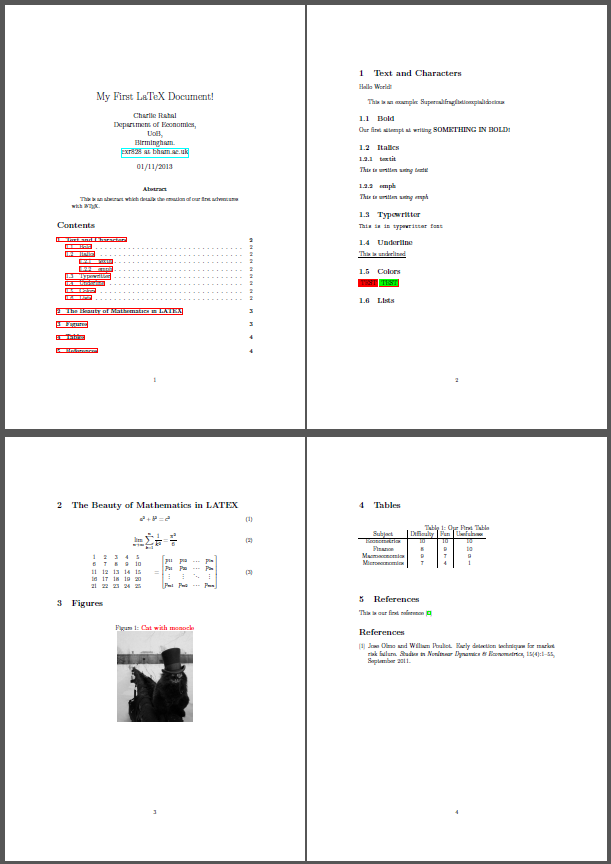
\includegraphics{endresult}}
\end{figure}
}

\frame{\frametitle{Stata and \LaTeX{} Integration!}
One request which I had from Dr. Pouliot was to show you how to convert Stata tables to \LaTeX. Let's quickly run through an example...\\
\begin{block}{eststo}
\begin{tt}
ssc install estout, replace\\
webuse auto\\
eststo: regress price weight mpg\\
eststo: regress price weight mpg foreign\\
esttab using example.tex\\
\end{tt}
\end{block}
This will then create an output \emph{.tex} file
}


\frame{\frametitle{Stata and \LaTeX{} Integration! (Cont.)}
Then we want to use the table we created (example.tex) in our document using the following commands.\\
\begin{center}
\footnotesize{
(Open a new file to try this, or put it at the end of \emph{myfirsttexfile.tex})}
\end{center}
\begin{block}{eststo}
\begin{tt}
$\backslash$documentclass\{article\}\\
$\backslash$begin\{document\}\\
$\backslash$input\{example.tex\}\\
$\backslash$end\{document\}\\
\end{tt}
\end{block}
}

\frame{\frametitle{Topics for Further Studies}
There are sadly many topics which we cannot cover in a brief two hour session when our intention is to get everybody to a functional level of \LaTeX{}...\\[0.1in]
\begin{enumerate}
\item Primarily, we would have wanted to consider other \emph{classes} such as Beamer.\\[0.1in]
\item In addition, we would have discussed a lot more packages, such as \emph{pdflscape} or how to set headers/footers.\\[0.1in]
\item One (ex-)PhD student even suggested we learn about the $\backslash$newcommand feature:
\begin{center}
$\backslash$newcommand\{name\}[num]\{definition\}
\end{center}
\item We would also have spoken alot about the error message window....
\end{enumerate}
}

\section{Nine}\label{nine}
\subsection{Outline and version control?}
\frame{\frametitle{Outline: GitHub}
An over-view of what we'll cover in this subsection of the course:\\[0.1in]
\begin{itemize}
\item Section \ref{nine}: Outline and version control?\\[0.1in]
\item Section \ref{ten}: An introduction to Git Bash \\[0.1in]
\item Section \ref{eleven}: An introduction to Git Hub\\[0.1in]
\item Section \ref{twelve}: Structure and commands \\[0.1in]
\item Section \ref{thirteen}: Branching and Pulling\\[0.1in]
\end{itemize}
}


\frame{\frametitle{GitHub: Support}
Three main sources for help:\\[0.1in]
\begin{enumerate}
\item GitHub documentation: \url{http://git-scm.com/doc}.\\[0.1in]
\item GitHub help: \url{http://help.github.com}.\\[0.1in]
\item Google and Stack Overflow are great resources.\\[0.1in]
\end{enumerate}
}


\frame{\frametitle{Version Control}
\begin{itemize}
\item Git is free, open source, distributed, and extremely efficient. \\[0.1in]
\item Git is the most popular type of `version control' system.\\[0.1in]
\item Everything is stored in local repositories (`repos').\\[0.1in]
\item A system that records all the changes you make to a file/set of files over time.\\[0.1in]
\item Extremely useful for collaboration.\\[0.1in]
\item A way to manage the work $\rightarrow$ save $\rightarrow$ change $\rightarrow$ save again cycle. \\[0.1in]
\end{itemize}
}

\frame{\frametitle{Downloading Git}
Find the download files which relate to your OS at:
\color{blue}
\begin{center}
\url{http://git-scm.com/downloads}
\end{center}
\color{black}
\begin{figure}
    \scalebox{.35}{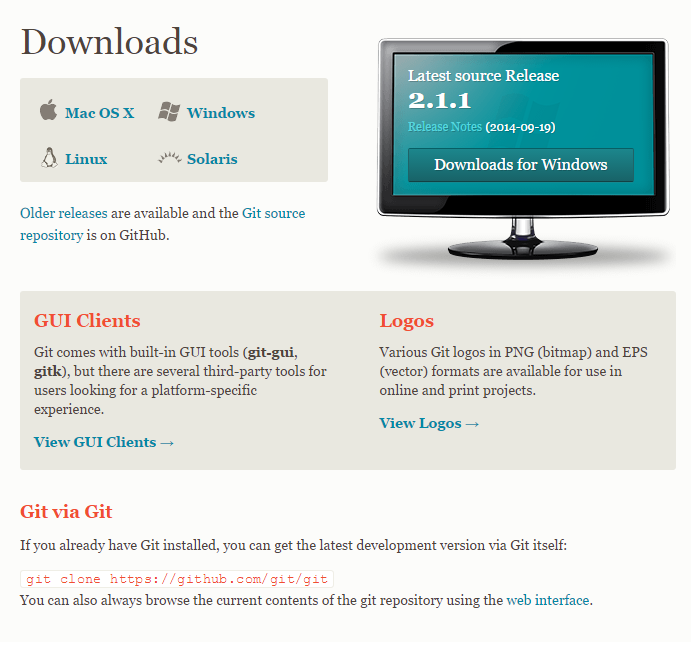
\includegraphics{gitdownload.png}}
\end{figure}
}

\section{Ten}\label{ten}
\subsection{An introduction to Git Bash}
\frame{\frametitle{Git Bash}
\begin{itemize}
\item The files are all the common standard of install files (e.g. .exe).\\[0.1in]
\item Default options simplest and best at the minute.\\[0.1in]
\item Then, open a program called Git Bash (search or look in Program Files $\rightarrow$ Git.\\[0.1in]
\item Dollar signs mean it's a prompt. You can also see your username/computer name.\\[0.1in] 
\item The first thing to do is to log in, as on the following slide $\hdots'$+:
\end{itemize}
}

\frame{\frametitle{Username and E-mail}
\begin{figure}
    \scalebox{.4}{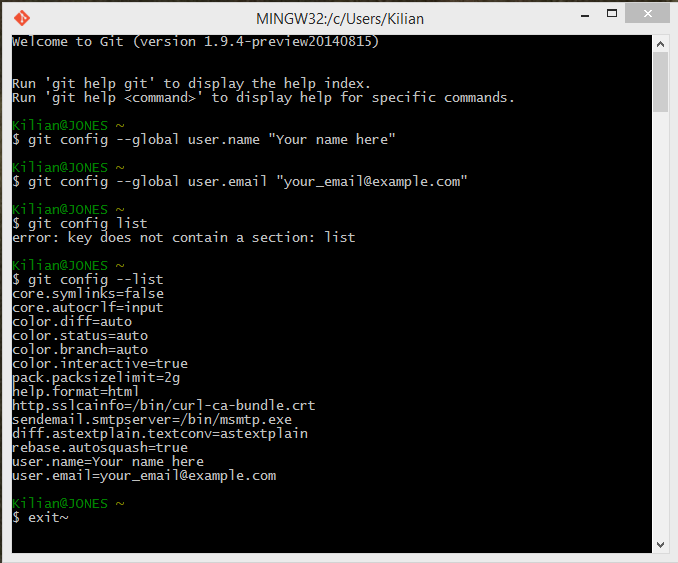
\includegraphics{gitbash}}
\end{figure}
}


\frame{\frametitle{Git}
\begin{itemize}
\item GitHub is a web based hosting service using Git revision control as a driving force.\\[0.1in]
\item Allows you to contribute to projects online, allowing you to also post your own projects.\\[0.1in]
\item Allows you to push and pull local repositories using Git on your local computer to remote repositories on the web.\\[0.1in]
\item Also provides you with a Git homepage (and gives you a backup of all your files).\\[0.1in]
\item The key is the social aspect: follow one another and share and collaborate and contribute.\\[0.1in]
\end{itemize}
}

\frame{\frametitle{Optional Review of Command Line Commands}
\begin{itemize}
\item \textbf{pwd:} Present working directory - what dir are you in?.\\[0.05in]
\item \textbf{clear:} Clears the screen.\\[0.05in]
\item \textbf{list:} Lists the files in your working directory.\\[0.05in]
\item \textbf{cd:} Changes your working directory.\\[0.05in]
\item \textbf{mkdir:} Creates a new directory.\\[0.05in]
\item \textbf{touch:} Creates a new file.\\[0.05in]
\item \textbf{cp:} Copies a file.\\[0.05in]
\item \textbf{rm:} Removes a file or directory if you use -r flag.\\[0.05in]
\item \textbf{mv:} Moving a file.\\[0.05in]
\item \textbf{date:} Check system date.\\[0.05in]
\item \textbf{echo:} Echo out a particular command.\\[0.05in]
\end{itemize}
}

\section{Eleven}\label{eleven}
\subsection{An introduction to Git Hub}
\frame{\frametitle{GitHub}
\begin{itemize}
\item Create your account at:
\color{blue}
\begin{center}
\url{http://git-scm.com/downloads}\\[0.1in]
\end{center}
\color{black}
\item Use the same e-mail as the one in the previous slide. You can also explore your profile page etc.\\[0.1in]
\item Documentation is extremely useful.\\[0.1in]
\item There are many guides to Git (Hub/Bash) on google as well, due to increasing popularity.\\[0.1in]
\end{itemize}
\begin{center}
\color{red}
\textbf{RECAP:} Git = Local (your computer), GitHub = Remote (web).
\color{black}
\end{center}
}


\frame{\frametitle{Starting a New Repo}
To start a new repo from scratch, we have two options:\\[0.1in]
\begin{enumerate}
\item Click `create new repo' on your profile page: \url{github.com/yourusername} and click on the top right corner.\\[0.1in]
\begin{center}
\textbf{OR}
\end{center}
\item GO directly to \url{github.com/new} when logged into your GitHub account.\\[0.1in]
\end{enumerate}
}

\frame{\frametitle{Starting a New Repo}
\begin{figure}
\caption{A New Repo}
    \scalebox{.225}{\includegraphics{newrepo}}
\end{figure}
Note: Private repos require a paid (or educational) account. Always initialize it with a README with a description of your repo. If you're interested, check out markdown files for your Repo.
}


\frame{\frametitle{Starting a New Repo}
Now we'll need to create a copy of this repo on your computer to make changes to it. Lets do this using Git Bash.
\begin{center}
\texttt{\$ mkdir $\sim$/test-repo}\\
\texttt{\$ cd $\sim$/test-repo}
\end{center}
Now initlize a local Git repository in this new directory:
\begin{center}
\texttt{\$git init}
\end{center}
Link up your local repo with your Git Hub repo with the URL e.g.:
\small
\begin{center}
\texttt{\$git remote add origin \url{https://github.com/yourusername/yourrepo-.git}}
\end{center}
}


\frame{\frametitle{Sync your Repo}
\begin{figure}
\caption{Initializing your Repo and Making it Available Offline}
    \scalebox{.55}{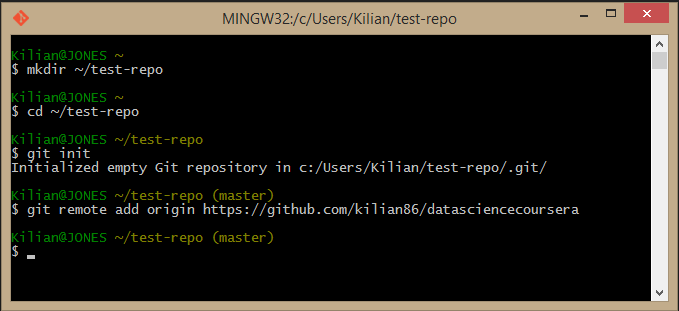
\includegraphics{syncrepo}}
\end{figure}
}

\frame{\frametitle{Fork a Repo}
\begin{itemize}
\item This is the second way to create a Repo. The idea is that you make a copy of somebody elses's repo.\\[0.1in]
\item Naviate to that repo online and click the `fork' button: creates a copy of this repo in your own profile.\\[0.1in]
\item You can make a local copy of this using the `clone' command e.g:\\[0.1in]
\small
\begin{center}
\texttt{\$ git clone https://github.com/yourusername/reponame.git}
\end{center}
\normalsize
\item This will clone to your PWD.
\item If you make changes to your copy: you'll want to push it back to Git Hub.\\[0.1in]
\end{itemize}
}
\section{Twelve}\label{twelve}
\subsection{Structure and commands}
\frame{\frametitle{Structure and Commands}
\begin{figure}
\caption{Pushing and Pulling}
    \scalebox{.25}{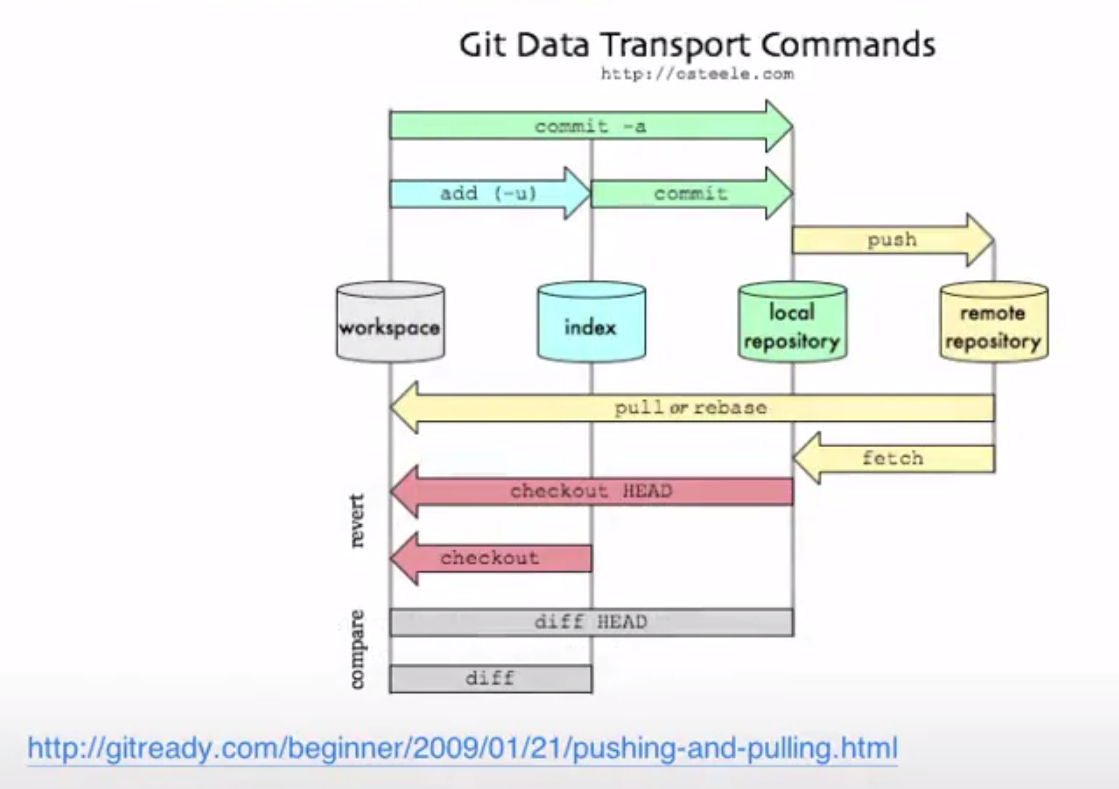
\includegraphics{gitpushpull}}
\end{figure}
}

\frame{\frametitle{The Git Layout}
\begin{itemize}
\item \textbf{Workspace:} Where you're working on your computer (directory).\\[0.1in]
\item \textbf{Index:} tells Git what files to control under version control.\\[0.1in]
\item \textbf{Local repository:} Files which are stored/version controlled on your computer.\\[0.1in]
\item \textbf{Remote repository:} In our case: Github.\\[0.1in]
\item Workspace $\rightarrow$ New File $\rightarrow$ Add file to index $\rightarrow$ Git knows to monitor file $\rightarrow$ Commit file to local repository so it can be stored/updated $\rightarrow$ push it to GitHub.\\[0.1in]
\end{itemize}
}

\frame{\frametitle{Basic Git Commands}
\begin{itemize}
\item Let Git know which files need to be tracked:
\end{itemize}
\begin{enumerate}
\item \texttt{git add .} - adds all new files in a directory.\\[0.1in]
\item \texttt{git add -u} - updates tracking for files that were changed/deleted.\\[0.1in]
\item \texttt{git add -A} - does both of the above.\\[0.1in]
\item \texttt{git commit -m ``message''} - commit changes to be saved as an intermediate version. Always use a message! (Note that this only updates your local repo, not your remote repo).\\[0.1in]
\item \texttt{git push} - put locally committed files/folders on GitHub.\\[0.1in]
\end{enumerate}
}

\section{Thirteen}\label{thirteen}
\subsection{Branching and Pulling}
\frame{\frametitle{Branches}
\begin{itemize}
\item Branching is useful for collaboration - you might not want to edit master version (because you'll break it!).\\[0.1in]
\item To create a branch:
\end{itemize}
\begin{enumerate}
\item \texttt{git checkout -b branchname} - create a new branch.\\[0.1in]
\item \texttt{git branch} - tells you what branch you're on.\\[0.1in]
\item \texttt{git checkout master} - lets you switch back to the master branch.\\[0.1in]
\end{enumerate}
}


\frame{\frametitle{Pull Request}
Once youve made a push to your remote repo on a branch, you can merge a branch or a fork back to the original repo/branch.
You can do this on the GitHub website: `Compare and Pull Request' gives notification to other users.
\begin{figure}
\caption{Pushing and Pulling}
    \scalebox{.25}{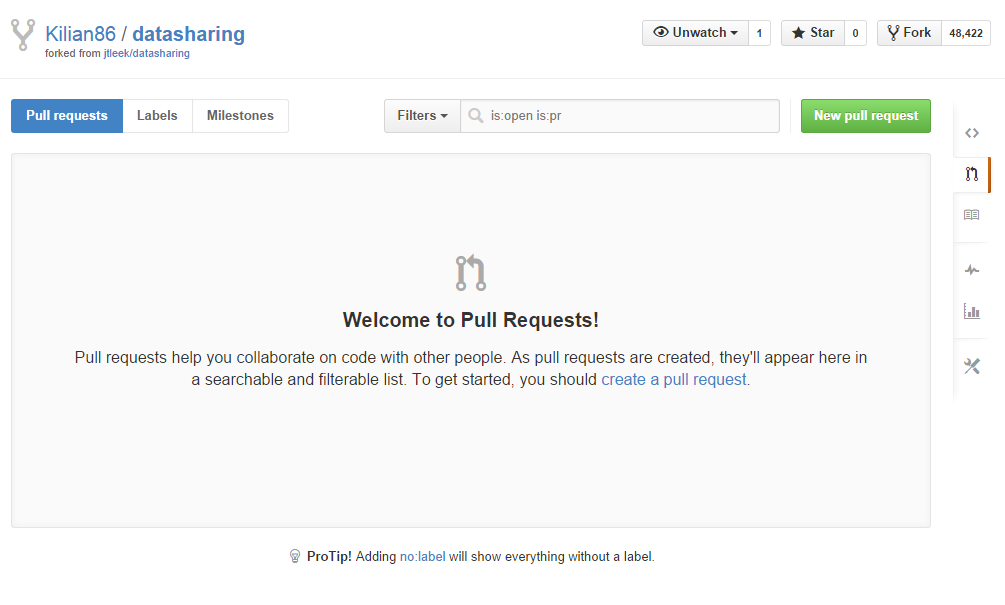
\includegraphics{gitpull}}
\end{figure}
}








\frame{\frametitle{Things To Practice On}
\begin{center}
\begin{alertblock}{Because Practice is Important!}
\begin{itemize}
\item Sign up for a GitHub account(!)\\[0.1in]
\item Make a .tex file for any of your coursework to be submitted this term, such as a micro assignment.\\[0.1in]
\item Prepare a presentation using the .beamer document class\\[0.1in]
\item Make a .do file of our Stata lecture last month and push it to your GitHub repo.
\end{itemize}
\end{alertblock}
\end{center}
}














\end{document}
